\documentclass[10pt]{article}
	\usepackage[margin=0.75in]{geometry}
\usepackage{amsmath, amsthm, amssymb}
\usepackage{mathtools}
\usepackage{url}
\usepackage{enumitem}
\usepackage{setspace}
\usepackage{scalefnt}
\usepackage[utf8]{inputenc}
\usepackage[english]{babel}
\usepackage{algorithm}
%\usepackage{algorithm2e}
%\usepackage{algorithmicx}
\usepackage[noend]{algpseudocode}
\usepackage{bbm}
\usepackage{graphicx}

\usepackage{hyperref} % load hyperref last

\newtheorem{theorem}{Theorem}
\newtheorem{definition}{Definition}
\newtheorem{proposition}{Proposition}
\newtheorem{lemma}{Lemma}
\newtheorem{corollary}{Corollary}
% \newcommand{\CommentX}[1]{\unskip~\%~#1~\%}

\DeclareMathOperator*{\argmax}{arg\,max}
\DeclareMathOperator*{\argmin}{arg\,min}
\DeclarePairedDelimiter\ceil{\lceil}{\rceil}
\DeclarePairedDelimiter\floor{\lfloor}{\rfloor}


\begin{document}

	\subsection*{Multidimensional persistence}
A natural question is whether or not there exists a multi-dimensional generalization of persistence. The starting point for this generalization is a structure which filters the space in multiple dimensions simultaneously, a \emph{multifiltration}. Our goal is to use such a structure to identify persistent features by examining the entire multifiltration. Such a generalization has been thought to have enormous potential in terms of applications~\cite{}. 
For example, one of the often noted drawbacks of persistence is its instability with respect to strong outliers. That is, although persistence diagrams are stable with respect to their input and thus are robust to noise, the presence of outliers can artificially introduce topological features such as loops, obscuring the persistence of significant topological features~\cite{buchet2015topological}. Indeed, this obfuscation can hinder the ability of 1D persistence to uncover ``significant'' topological features, notably one of the most important applications of persistence. In theory, this formalism enables the practitioner to analyze even noisy data sets directly without resorting to sophisticated data preprocessing techniques which may or may not preserve the underlying topology of the data. 

Unfortunately, invariants related to multidimensional persistence have proven challenging to use in practice due to the high algorithmic complexity of their corresponding computation. A number of computational strategies have been proposed to counter this, such as homology preserving multi-filtration simplification or parallelization schemes using shared-memory computation~\cite{}. Another strategy is to focus specifically on the case of 2-D persistence. Utilizing the equivalence between the rank and fibered barcode invariants, Lesnick and Wright~\cite{} developed an elegant way of computing the former via a reparameterization of the latter using standard point-line duality. This clever reparameterization reduces the computation of the rank invariant to sequence of 1-D barcode computations at ``template points'' lying within the 2-cells of particular planar subdivision of the half-plane $[0, \infty) \times \mathbb{R}$. 

%Indeed, since algorithm~\ref{alg:schedule} was designed for precisely such a computation, the algorithm proposed by~\cite{lesnick2015interactive} is prototypical of the class of methods that stand to benefit from move scheduling. In what follows, we briefly recount this reparameterization 

% --- For each section of the paper, consider writing a mini-introduction that says what its organization is, what is in each subpart, and how the parts relate to one another.

%To demonstrate how our scheduling approach can accelerate the multidimensional persistence computation, we establish the computational framework we will be considering. 
% These transforms end up being crucial in decomposing the definition of the fibered barcode (and thus, the rank invariant) into a discrete computation.

\subsubsection*{The Rank Invariant}

%We begin with a few definitions. An $n-D$ \emph{filtration} is a functor $\mathcal{F} : \mathbb{R}^n \to \textbf{Simp}$, the category of simplicial complexes, such that for all $a \leq b$, $\mathcal{F}(a,b) : F_a \to F_b$ is an inclusion. We will focus exclusively on the case where $n = 2$, where the object of study is a \emph{bifiltration}. Multifiltrations can be broadly categorized into two types: 1-critical and multi-critical filtrations. A \emph{1-critical filtration} $\mathcal{F}$ is a finite $n-D$ filtration each simplex $s \in K$ is associated with only one multi-grade (denoting its appearance in each of the filtered dimensions), otherwise $\mathcal{F}$ is said to \emph{multi-critical}. 
%An $n-D$ persistence module is a functor $M : \mathbb{R}^n \to \textbf{Vect}$, where $\textbf{Vect}$ denotes the category of $\mathbf{F}$-vector spaces and linear maps for some suitable field $\mathbb{F}$. A module $M$ is said to be \emph{pointwise finite dimensional} (p.f.d) if $\mathrm{dim}(M_a) < \infty$ for all $a \in \mathbb{R}^n$.
%For $i \geq 0$, let $H_i : \textbf{Simp} \to \textbf{Vect}$ denote the $i^{\text{th}}$ simplicial homology functor with coefficients in $\mathbb{F}$. 
%Using this notation, given a 1D filtration $\mathcal{F}$ of size $m$, each p.f.d 1D persistence module $M = H_i(\mathcal{F})$ for  may be associated with a multiset $\mathcal{B}(M)$ of intervals in $\mathbb{R}$ which record the isomorphism classes of indecomposable summands of $M$. The set $\mathcal{B}(M)$ is called the \emph{barcode}\footnote{Note that \emph{barcodes} and \emph{persistence diagrams} are interchangeable representations of the same multiset.} of $M$.

An \emph{invariant} of $n$-parameter persistence modules is a function from the collection of persistence modules to some set $S$ with the property that $f(M) = f(M')$ when $M \cong M'$. An invariant is said to be \emph{complete} if $M \cong M'$ whenever $f(M) = f(M')$. Thus, incomplete invariants are invariants which may have the same value on two non-isomorphic modules. 
\emph{The rank invariant} proposed by Carlsson et al~\cite{carlsson2009theory} is one such invariant that is complete when $n=1$ but is otherwise incomplete when $n \geq 2$. 
% The rank invariant is computable in polynomial time~\cite{carlsson2010computing}, that has been the subject of much interest lately. 
It is defined as follows: 
\begin{definition}[Rank Invariant]
	For $n \geq 1$, the \emph{rank invariant} of a $\mathbb{R}^n$-indexed persistence module $M$ over $\mathcal{H}^{n} \subseteq \mathbb{R}^n \times \mathbb{R}^n$ is the function:
	\begin{equation*}
		\begin{aligned}
		& \mathrm{rank}(M)  \; : & \mathcal{H}^n & \to \mathbb{N}  \\
		& & (a,b) & \mapsto \mathrm{rank} \, M(a,b) 
		\end{aligned}
	\end{equation*}
	for $a \leq b \in \mathcal{H}^n$. When $n = 1$, the rank invariant is complete, thus $\mathrm{rank}(M)$ and the persistence barcodes $\mathcal{B}(M)$ determine each other.
\end{definition}
\noindent Thus, in one dimension, persistent homology provides a complete invariant that fully captures the lifetime of topological features in a given filtration: 1-D persistent homology modules decompose in an essentially unique way into indecomposable summands~\cite{zomorodian2005computing}. In contrast, the theory of multidimensional persistence shows that no complete discrete invariant exists---the structure of the target for the invariant depends on the structure of the underlying field, and although multiparameter persistence modules also decompose in a similar way as the 1-D case, the set of isomorphism classes is known to be extremely complicated~\cite{carlsson2009theory, lesnick2015interactive}. 
Nonetheless, there are invariants related to multi-parameter persistence that can be quite useful in practice, even though they are incomplete. 
\noindent For example, even though the rank invariant does not encode the isomorphism type of the underlying module $M$ when $n > 1$, it does captures important ``first-order'' information about the modules structure. 

Along this vein of research, Lesnick and Wright~\cite{lesnick2015interactive} identify three simple invariants associated with a multidimensional persistence module $M$: the \emph{dimension function of $M$}, the \emph{multigraded Betti numbers of $M$}, and the \emph{fibered barcode of $M$}. 
% The dimension function is simply the the function which maps every point $a \in \mathbb{R}^2$ to $\mathrm{dim}(M_a)$. It is a simple and easy to visualize invariant, but is unstable and yields no information about the persistent features of $M$. 
% The multigraded Betti numbers constitute a natural and important class of invariants associated with a multidimensional persistence module. There are many ways of defining these, with perhaps the simplest definition stemming from minimal resolutions: for a finitely generated $n$-parameter persistence module $M$ and $i \in \{0, 1, \dots, d \}$, the $i^{\text{th}}$ graded Betti number of $M$ at grade $z$, denoted as $\xi_i^M(z)$, is defined as the number of elements at grade $z$ in a basis of the $i^{\text{th}}$ module in a free resolution for $M$. 
% Thus, the $i^{\text{th}}$-graded Betti number of $M$ is a function $\xi_i(M): \mathbb{R}^n \to \mathbb{N}$. Being central objects in commutative algebra and algebraic geometry, both the theory and the computation of multi-graded Betti numbers is extensive and beyond the scope of this effort---the interested reader is referred to~\cite{carlsson2009theory, lesnick2015interactive} for more details. 
The fibered barcode, denoted as $\mathcal{B}(M)$, is defined as follows: 
\begin{definition}[Fibered barcode]
	%\in \overline{\mathcal{L}}
	The fibered barcode $\mathcal{B}(M)$ of a bipersistence module $M$ is the map which sends each line $L$ with non-negative slope to the barcode $\mathcal{B}_L(M)$: 
	$$ L \mapsto \mathcal{B}_L(M) $$
	Thus, the fibered barcode is simply a 2-parameter family of barcodes given by the collection of 1-D affine slices of $M$. 
\end{definition} 
\noindent Each line $L$ induces a 1-parameter restriction on $M$. The fibered barcode enjoys a number of stability properties readily expressed using interleaving distances, see~\cite{}. More important to this work, the fibered barcode $\mathcal{B}(M)$ and the rank invariant $\mathrm{rank}(M)$ determine each other~\cite{}. 

\subsubsection*{Fibered barcode reparameterization}
Let $\overline{\mathcal{L}}$ denote the collection of all lines in $\mathbb{R}^2$ with non-negative slope, $\mathcal{L} \subset \overline{\mathcal{L}}$ the collection of all lines in $\mathbb{R}^2$ with non-negative, finite slope, and $\mathcal{L}^\circ$ the collection of all affine lines in $\mathbb{R}^2$ with positive, finite slope. There is a standard point-line duality that gives a parameterization of $\mathcal{L}$ with the half-plane $[0, \infty) \times \mathbb{R}$ that is convenient to work with here. Define the \emph{line} and \emph{point} dual transforms $\mathcal{D}_{\ell}$ and $\mathcal{D}_p$, respectively, as follows: 
\begin{equation}
	\begin{aligned}
\mathcal{D}_{\ell}: \mathcal{L} \rightarrow[0, \infty) \times \mathbb{R} & \quad \hfill \quad & \mathcal{D}_{p}:[0, \infty) \times \mathbb{R} \rightarrow \mathcal{L} \\
y=a x+b \mapsto(a,-b) &\quad \hfill \quad & (c, d) \mapsto y=c x-d
\end{aligned}
\end{equation}
% Use \multicolumn{1}{|r|}{text} to align
The transforms $\mathcal{D}_{\ell}$ and $\mathcal{D}_p$ are \emph{dual} to each other in the sense that for any point $a \in [0, \infty) \times \mathbb{R}$ and any line $L \in \mathcal{L}$, $a \in L$ if and only if $D_\ell(L) \in D_{p}(a)$. Now, for some fixed line $L$, define  the \emph{push map} $\mathrm{push}_L(a):  \mathbb{R}^2 \to L \cup \infty$ as: 
\begin{equation}
	\mathrm{push}_L(a) \mapsto \mathrm{min}\{ v \in L \mid a \leq v \}
\end{equation}
%\begin{equation*}
%	\begin{aligned}
%	& \mathrm{push}_L : & \mathbb{R}^2 & \to L \cup \infty \\
%	& & a \in \mathbb{R}^2 & \mapsto \mathrm{min}\{ v \in L \mid a \leq v \}
%	\end{aligned}
%\end{equation*}
The push map satisfies a number of useful properties. Namely: 
\begin{enumerate}
	\item For $r < s \in \mathbb{R}^2$, $\mathrm{push}_L(r) \leq \mathrm{push}_L(s)$
	\item For each $a \in \mathbb{R}^2$, $\mathrm{push}_L(a)$ is continuous on $\mathcal{L}^\circ$
	\item For $L \in \mathcal{L}^\circ$ and $S \subset \mathbb{R}^2$, $\mathrm{push}_L$ induces a totally ordered partition $S_L$ on $S$ 
\end{enumerate}
Property (1) asserts that for any $L \in \overline{\mathcal{L}}$, the partial order on $\mathbb{R}^2$ restricts to a total order on $L$. Properties (2) and (3) qualify the following definition:
\begin{definition}[Critical Lines]
	For some fixed $S \subset \mathbb{R}^2$, a line $L \in L^\circ$ is defined to be \emph{regular} if there is an open ball $B \in L^\circ$ containing $L$ such that $S_L = S_{L'}$ for all $L' \in B$. Otherwise, the line $L$ is defined as \emph{critical}. 
\end{definition}
\noindent The set of critical lines $\mathrm{crit}(M)$ with respect to some fixed set $S \subset \mathbb{R}^2$ fully characterizes a certain planar subdivision of the half plane $[0, \infty) \times \mathbb{R}$. Explicitly, define $\mathcal{A}^1(M)$ to the 1-skeleton of the line arrangement defined by: 
% \{ \mathcal{D}_p(\alpha) \text{ for } \alpha = \mathrm{LUB}(u,v), u,v \in S \} 
\begin{equation}\label{eq:arrangement_crit}
	\mathcal{A}^1(M) = \{ \mathcal{D}_{\ell}(\mathrm{crit}(M)) \cup (\{0\} \times \mathbb{R}) \}
\end{equation}
Expanding the 1-skeleton to a 2-D cell complex $\mathcal{A}(M)$ fully partitions the upper half plane.  
A consequence of equation~\ref{eq:arrangement_crit} that if the duals of two lines $L, L' \in \mathcal{L}$ are contained in the same $2$-cell in $\mathcal{A}(M)$, then $S_L = S_{L'}$, i.e. the partitions induced by $\mathrm{push}_L$ are equivalent. Indeed, the total order on $S_L$ is the pullback of the total order on $L$ with respect to the push map.
Since $\mathcal{A}(M)$ partitions the entire half-plane, the dual to every line $L \in \mathcal{L}$ is contained within $\mathcal{A}(M)$---the desired reparameterization. 

Let $S = \mathrm{supp}\,\xi_0(M) \, \cup \, \mathrm{supp}\,\xi_1(M)$, where the functions $\xi_0(M), \xi_1(M)$ are $0^{\text{th}}$ and $1^{\text{st}}$ bigraded Betti numbers of $M$, respectively. 
The main mathematical result from~\cite{lesnick2015interactive} is a characterization of the barcodes $\mathcal{B}_L(M)$, for any $L \in \mathcal{L}$, in terms of a set of \emph{barcode templates} $\mathcal{T}$ computed at every 2-cell in $\mathcal{A}(M)$.
 More formally, for any line $L \in \overline{\mathcal{L}}$ and $e$ any 2-cell in $\mathcal{A}(M)$ whose closure contains the dual of $L$ under point-line duality, the 1-parameter restriction of the persistence module $M$ induced by $L$ is given by: 
 \begin{equation}
 \mathcal{B}_L(M) = \{ [\,\mathrm{push}_L(a), \, \mathrm{push}_L(b)\,) \mid (a,b) \in \mathcal{T}^e, \mathrm{push}_L(a) < \mathrm{push}_L(b)  \} 
\end{equation}
Minor additional conditions are needed for handling completely horizontal and vertical lines. 
The importance of this theorem for this effort lies in the fact that the fibered barcodes are completely defined from the precomputed barcode templates $\mathcal{T}$: once $\mathcal{T}$ has been computed and augmented onto $\mathcal{A}(M)$, $\mathcal{B}(M)$ is completely characterized, and the barcodes $\mathcal{B}_L(M)$ of any $L$-induced 1-D filtration can be efficiently computed via a point-location query on $\mathcal{A}(M)$ and a $O(\lvert \mathcal{B}_L(M) \rvert)$ application of the push map.

	\begin{figure}[h]
	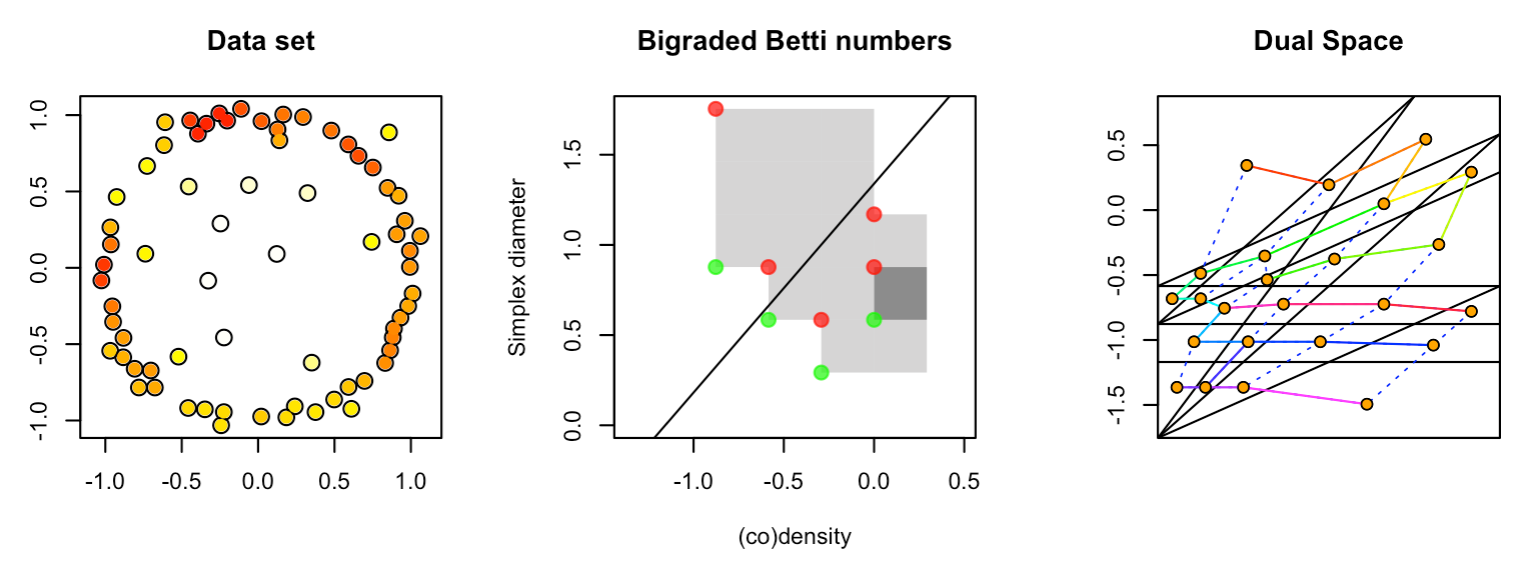
\includegraphics[width=0.98\textwidth]{bifiltration_ex2}
	\caption{Bipersistence example on an $8 \times 8$ coarsened grid. On left, the input data, colored by density. In the middle, the bigraded Betti numbers $\xi_0(M)$ and $\xi_1(M)$ (green and red, respectively), the Hilbert function (gray), and a line $L$ emphasizing the persistence of features with high density. On the right, the line arrangement $\mathcal{A}(M)$ lying in the dual space $D_p(\alpha)$ derived from the $\xi(M)$. The barycenters of the 2-cells in $\mathcal{A}(M)$ depicting where the barcodes templates $\mathcal{T}$ are computed are drawn as orange points, and the dual graph $G$ of $\mathcal{A}(M)$ is drawn using dotted blue lines. The eulerian path through $G$ is shown by the solid colored lines. }
\end{figure}

\end{document}